\documentclass[11pt, a4paper, spanish, openright, twoside]{book}
\usepackage[spanish, activeacute]{babel}
\usepackage[utf8]{inputenc}
%\usepackage[top=2.5cm, bottom=2.5cm, outer=1.75cm, inner=1.75cm, heightrounded, marginparwidth=2.5cm, marginparsep=0.3cm]{geometry}	%márgenes empequeñecidos
\usepackage[top=2.95cm, bottom=2.25cm, outer=2.75cm, inner=2.75cm, heightrounded, marginparwidth=2.5cm, marginparsep=0.3cm]{geometry}	%márgenes originalmente
\usepackage{dpg}
\usepackage{fli}

\usepackage{pgf}
\usepackage{tikz}

\usepgflibrary{shapes.geometric} % LATEX and plain TEX and pure pgf
\usetikzlibrary{arrows,automata,positioning}
\tikzstyle{accepting by double}= [double distance=1.6pt,double,outer sep=.5\pgflinewidth+.8pt] % esto es algo estético.
\renewcommand\shorthandsspanish{}  % para compatibilizar spanish con tikz

%%%%%%		Figuras		%%%%%%%%%%%%%%%%%%%
\usepackage[vflt]{floatflt}		%Entorno float-figure

%%%%%%		Page style		%%%%%%%%%%%%%%%%%%%
\renewcommand{\thepage}{\arabic{page}}% Arabic page numbers\fancyhead{}
\pagestyle{fancy}
\fancyfoot{}
\fancyhead[LO,RE]{Práctica 11}	%encabezado de pares: nombre de la sección
\fancyhead[RO,LE]{Aprendizaje automático con WEKA}
\fancyfoot[LE,RO]{\thepage}	%abajo a izqda en pares, derecha en impares: numero de pagina
%\fancyhead[LE]{\nouppercase{\leftmark}} %cuadro izquierdo de pagina par: parte y contador
\fancyfoot[CE]{Inteligencia Artificial} 
\fancyfoot[CO]{Doble Grado Informática-Matemáticas - Universidad Complutense}
\renewcommand{\footrulewidth}{0.4pt}
\renewcommand{\headrulewidth}{0.4pt}		% linea por debajo del encabezado
\renewcommand{\sectionmark}[1]{\markright{\textbf{\thesection. #1}}}	%negrita
\renewcommand{\labelitemi}{$\circ$} %Primer itemize con circunferencia vacia
\renewcommand{\labelitemii}{$\cdot$} %Segundo itemize con punto pequeño \cdot
\renewcommand*{\thesection}{\arabic{section}}	% Hace que no apareca el indice de capitulos y que comience en section

%%%%%%		Others		%%%%%%%%%%%%%%%%%%%
\setlength{\leftmarginii}{0em} %Segundo itemize sin sangria
\setlength{\leftmarginiii}{1em} %Tercer itemize casi sin sangria
\renewcommand{\labelitemiii}{ }
\pagenumbering{roman}
\addto{\captionsspanish}{\renewcommand*{\contentsname}{Índice}} %Cambia "Indice general" por "Indice"



\begin{document} 
\title{\Huge{\textsc{Inteligencia Artificial}} \\
	\vspace{0.7cm}
	 \textsc{\Large{Práctica 11}} \\
	\vspace{1.5cm}
	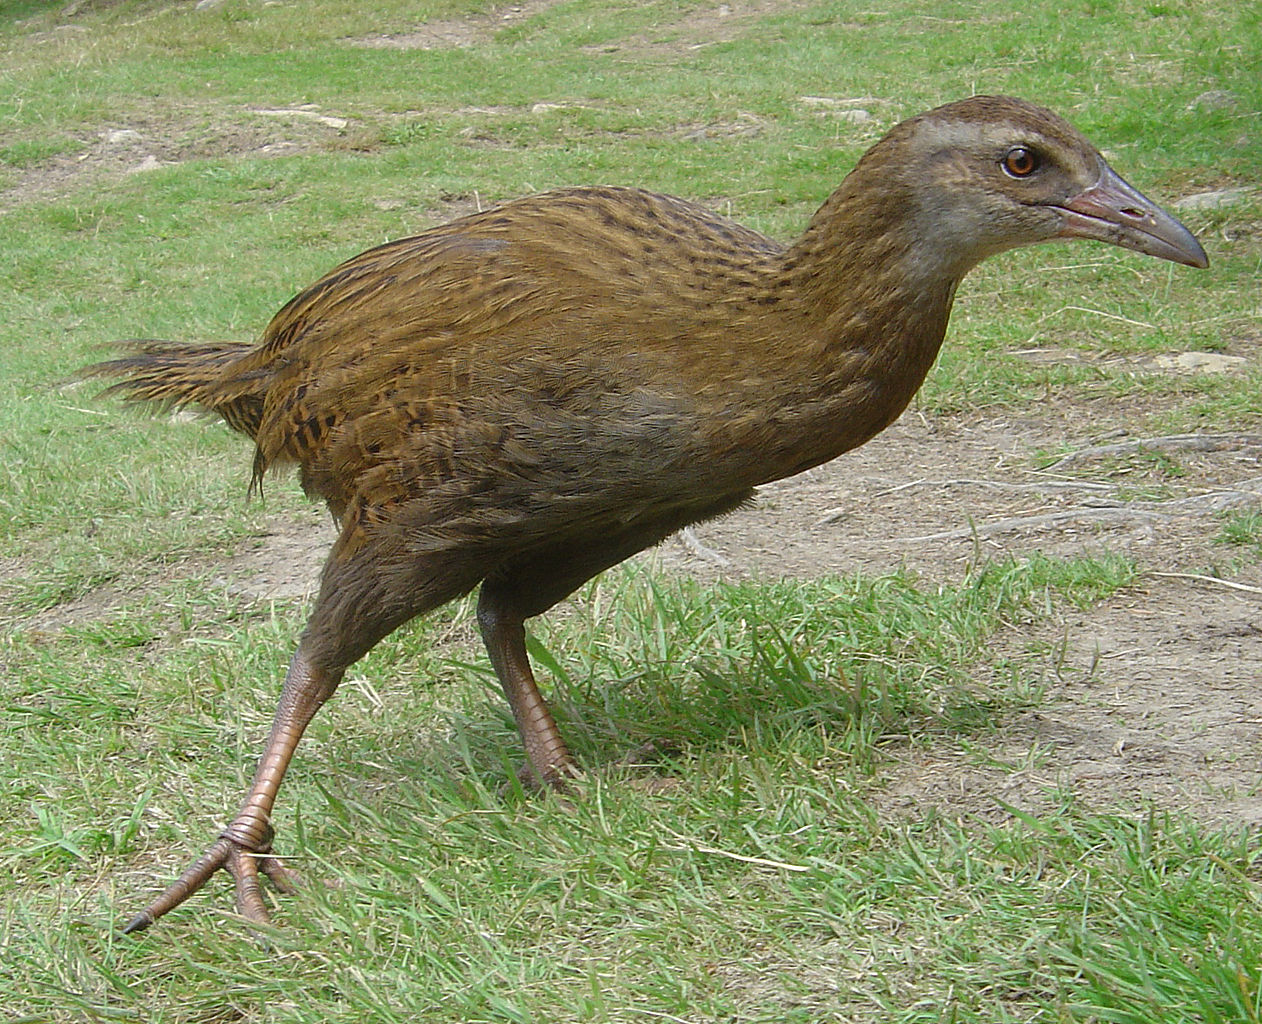
\includegraphics[scale=0.2]{weka}
	}
\author{\textsc{Grupo 3:}\\
	Enrique Ballesteros Horcajo\\
	Ignacio Iker Prado Rujas}
\date{\Today}
\maketitle

\newpage
\mbox{}
\thispagestyle{empty}						% Hoja en blanco, sin numeros ni nada
\newpage


\tableofcontents 							%INDICE hipervinculado

\newpage
\mbox{}
\thispagestyle{empty}						% Hoja en blanco, sin numeros ni nada
\newpage

\pagenumbering{arabic}						% Pone el contador de paginas a 1 y ahora en numeros normales

\vspace{3cm}


\newpage

\begin{section}{Introducción}
	
	En esta práctica vamos a trabajar con el entorno que nos proporciona WEKA\footnote{Página web de WEKA \href{http://www.cs.waikato.ac.nz/ml/weka/}{aquí}.}, aplicando herramientas de aprendizaje automático a conjuntos de datos dados por los ficheros \texttt{diabetes.arff} y \texttt{glass.arff}.
	
\end{section}

\begin{section}{Apartado 1}
	Tabla 4x4. Ordenar con itemize o lo que sea para que quede elegante. 
	
	 Analiza el archivo citado y contesta las siguientes preguntas: ¿Cuántas instancias hay? ¿Cuántos 
atributos se utilizan? ¿Por qué atributo queremos aprender a clasificar? 
- Ejecuta J48 (versión WEKA de C4.5). Utiliza para la validación el “training set”. Incluye en la 
memoria los resultados obtenidos y la representación gráfica del árbol correspondiente. ¿Cuántas 
instancias han sido mal clasificadas? ¿Cuántos nodos terminales hay en el árbol? ¿Por qué atributo 
se clasifica en el primer nivel del árbol? 
- Vuelve a ejecutar J48 primero con "cross-validation" y después con "percentage split" (con un valor 
del 66\%) y observa las diferencias. Haz una tabla con el porcentaje de instancias bien clasificadas en 
cada uno de los tres métodos de validación. Incluye en esa tabla la precisión y el recall para cada 
uno de los tres métodos. Comenta los resultados obtenidos. ¿Cuál de las tres validaciones te parece 
más fiable? ¿Por qué? ¿Cuántos falsos negativos (FN) y falsos positivos (FP) se han obtenido con el 
“percentage split”? 

\end{section}

\begin{section}{Apartado 2}
	Analiza el dataset. ¿En cuántas clases se clasifican los ejemplares? ¿Cuántos atributos se utilizan? 
- Aplica el clustering jerárquico a este conjunto de datos para 7 clusters y comenta los resultados 
obtenidos. ¿Qué clases han quedado mejor clasificadas? 
- Discretiza los atributos utilizando un filtro supervisado. ¿Qué horquillas se han generado para los 
valores del Calcio? Vuelve a ejecutar el clustering jerárquico y compara los resultados con los 
anteriores. ¿Qué clases han quedado mejor clasificadas? 
- Con los atributos en su estado original, utiliza el algoritmo de clustering EM (Expectation 
Maximization) y compara con los resultados anteriores. ¿Qué clases han quedado mejor 
clasificadas? ¿Qué método de los tres anteriores te parece más útil para este ejemplo? ¿Por qué? 
¿Podríamos haber utilizado un algoritmo de clasificación como J48? ¿Qué habríamos obtenido con 
los algoritmos de clustering si no tuviéramos el atributo de clase? ¿En qué casos sólo podríamos 
utilizar clustering?
\end{section}

	
\begin{thebibliography}{9}

\bibitem{aima}
	Russell, S.; Norvig, P, \\
	\emph{Artificial Intelligence, a modern aproach}.\\
	New Jersey: Pearson, 2010.
	
\bibitem{clase}
	Apuntes y transparencias de Inteligencia Artificial, \\
	Doble Grado Matemáticas - Ing. Informática, U.C.M., 2014-2015.

\end{thebibliography}


\end{document}